\chapter{Results
  \label{chap:result}}

%\subsection{Transitions}
The data obtained for CH$_{3}$NH$_{2}$ are summarized in Table \ref{tab:MAOri}.
Here the rest frequencies, product of the line strength and the dipole moment ($S\mu^2$), the upper state energy ($E_{\mathrm{u}}$), the quantum numbers,
the peak brightness temperature, the systemic velocity (V$_{\mathrm{LSR}}$) , and noise level are listed.

Out of 24 selected transitions in our observational frequency range, 
6 were probably identified and are reported in Table \ref{tab:MAOri}. 
The remaining 18 CH$_{3}$NH$_{2}$ transitions are blended with or masked by other spectral features, 
or its signal are below the noise level (See Appendix~B). 

\renewcommand{\arraystretch}{1.5}
\begin{table}[htb]
\begin{center}

  \caption{Observed rotational transitions of CH$_3$NH$_2$ in Orion-KL}
  \label{tab:MAOri}
{\scriptsize
  \begin{tabular}{cccccl} \hline
   Fequency [GHz]& S$\mu ^{2}$ [D$^2$] & E$_{\rm{u}}$ [K]& Transition ($J$, $K_{\rm{a}}$, $\Gamma$) & Noise [K]  &Comments \\ \hline 
    217.758 & 129.88 & 182.05 & 12, 2, $B_{2}$ $\rightarrow$ 12, 1, $B_{1}$ &  0.034 &Reported in Pagani+17 \\
    245.202 & 37.84 & 168.31 & 12, 1, $B_{2}$ $\rightarrow$ 11, 2, $B_{1}$ & 0.037 &Reported in Pagani+17 \\
    235.735 & 82.06 & 92.76 & 8, 2, $B_{2}$ $\rightarrow$ 8, 1, $B_{1}$ &  0.081 &Reported in Pagani+17 \\
    229.908 & 27.37 & 92.71 & 8, 2, $A_{2}$ $\rightarrow$ 8, 1, $A_{1}$ & 0.064&\\ 
    242.262 & 60.23 & 60.86 & 6, 2, $B_{2}$ $\rightarrow$ 6, 1, $B_{1}$ &  0.166 &SV data \\
    244.887 & 49.54 & 48.09 & 5, 2, $B_{1}$ $\rightarrow$ 5, 1, $B_{2}$ & 0.043 &Reported in Pagani+17 \\ \hline
  \end{tabular}
  }
\end{center}
\end{table}

\newpage
\section{Overall CH$_3$NH$_2$ distribution}
CH$_3$NH$_2$ emission appears mainly at Hot core and partially at IRc7 (Figure \ref{fig:mom0s}).
According to previous work \citep[see e.g.,][]{Feng+2015, Gong+2015}, N-bearing species tend to have 
similar peak at or near Hot core.  CH$_3$NH$_2$ also shows the same trend.

Figure \ref{ch_0}-\ref{ch_5} show channel maps of expected unblended lines at 217.758~GHz, 
245.202~GHz, 229.908~GHz, 235.735~GHz, 242.262~GHz, 244.887~GHz, respectively.
The channel maps enable us to confirm the region where the radiations of molecules come and its velocity component.

In the integrated intensity map of 229.908 GHz line, emission come from the southern part of Hot core.
Since it can be confirmed that the velocity component is different in the channel map (see Figure \ref{ch_3}), 
this is considered to be the emission of another molecular line.

In addition, the extended emission in Hot core and the compact structure at Compact ridge are seen 
in the integrated intensity map of 242.262 GHz line. These are also considered to be emission from other molecule line 
by the channel map (Figure \ref{ch_4}) and spectrum (Figure \ref{fig:spec}).

\newpage
%%%%% 積分強度図挿入 %%%%%
\begin{figure}[H] 
\begin{center}
\begin{minipage}{0.98\textwidth} 
\begin{center}
%%%% ここから
\begin{minipage}{0.48\textwidth}
\begin{center}
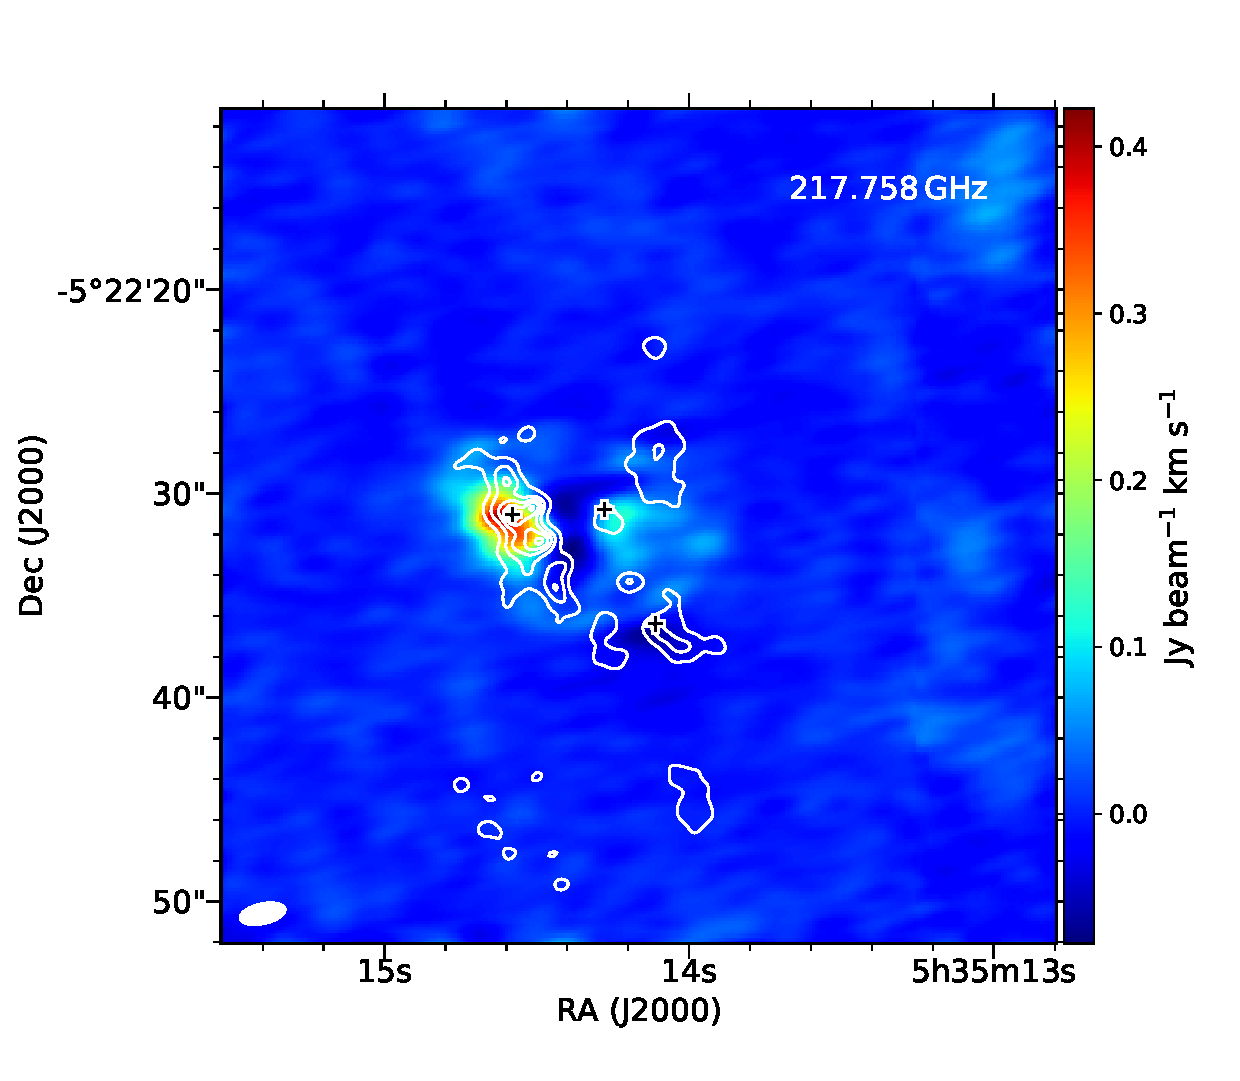
\includegraphics[width=0.98\textwidth]{OrionKL/mom0/217.758mom0_3-7.eps}
%\\(a) 左の図の説明
\end{center}
\end{minipage}
\begin{minipage}{0.48\textwidth}
\begin{center}
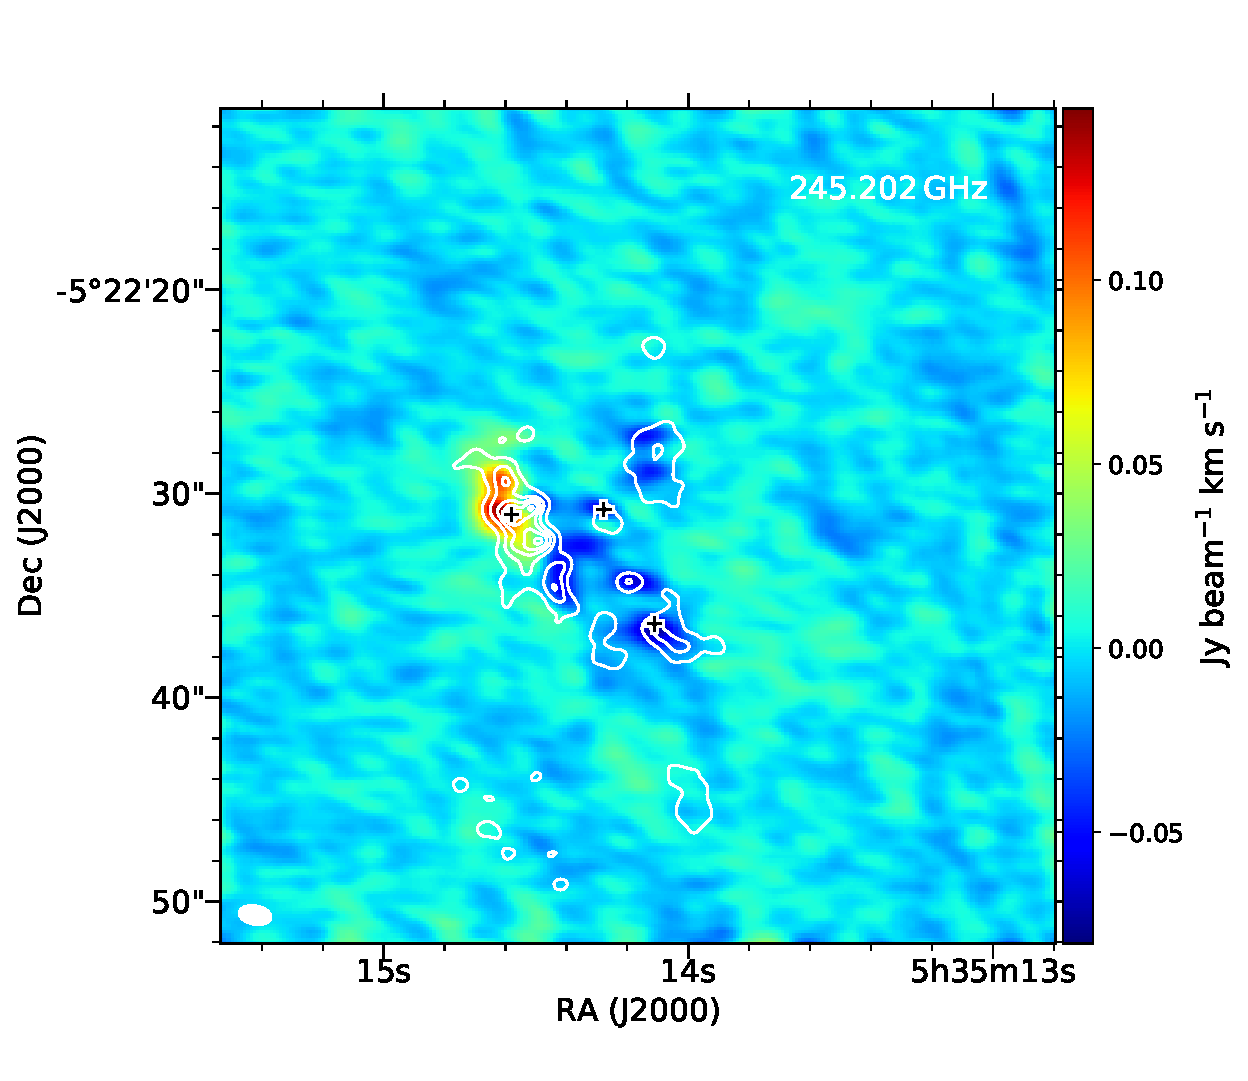
\includegraphics[width=0.98\textwidth]{OrionKL/mom0/245.202mom0_3-7.eps}
%\\(b) 右の図の説明
\end{center}
\end{minipage}
\end{center}
\end{minipage}
%%%% ここまで一組

%\begin{minipage}{0.98\textwidth} 
%\begin{center}
%\begin{minipage}{0.48\textwidth}
%\begin{center}
%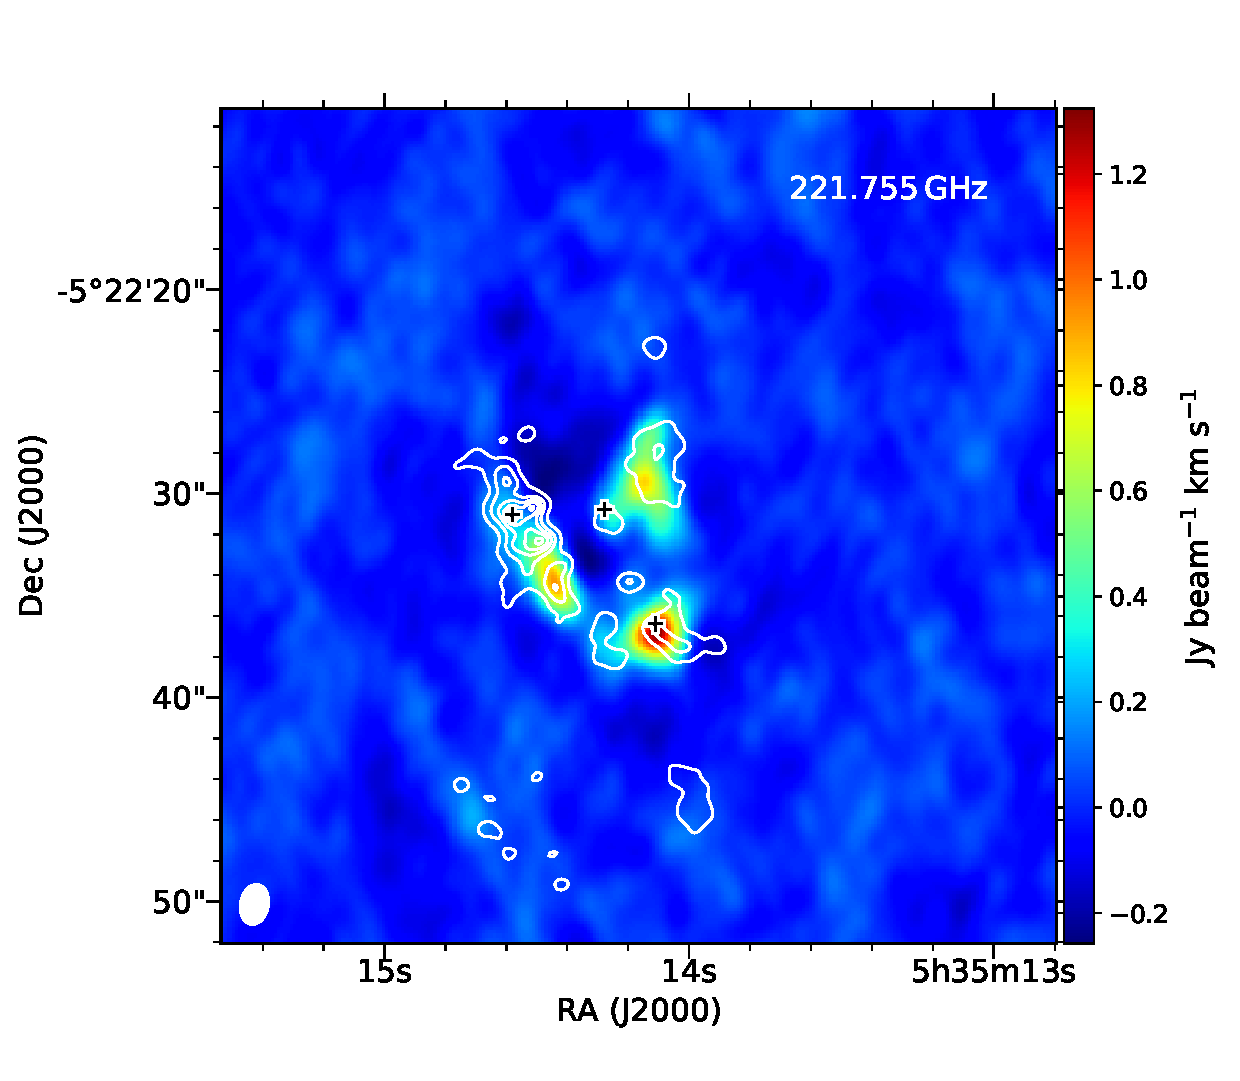
\includegraphics[width=0.98\textwidth]{OrionKL/mom0/221.755SV_mom0_3-7.eps}
%\\(c) 左の図の説明
%\end{center}
%\end{minipage}
%\begin{minipage}{0.48\textwidth}
%\begin{center}
%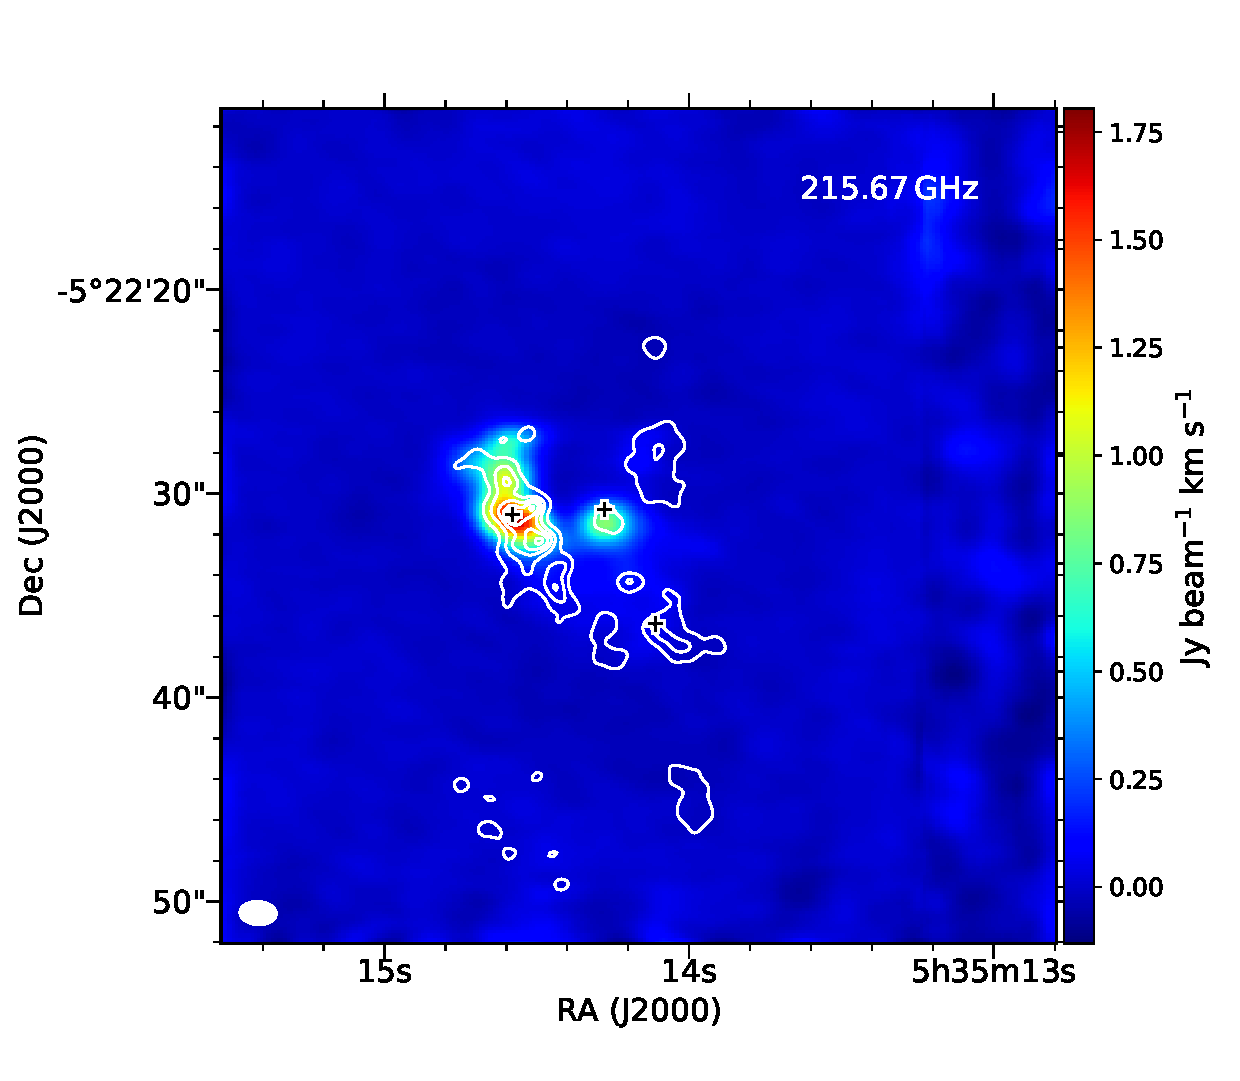
\includegraphics[width=0.98\textwidth]{OrionKL/mom0/215.67mom0_3-7.eps}
%\\(d) 右の図の説明
%\end{center}
%\end{minipage}
%\end{center}
%\end{minipage}
%\end{center}
%\end{figure}

%\begin{figure}[H] 
%\begin{center}
\begin{minipage}{0.98\textwidth} 
\begin{center}
%%%% ここから
\begin{minipage}{0.48\textwidth}
\begin{center}
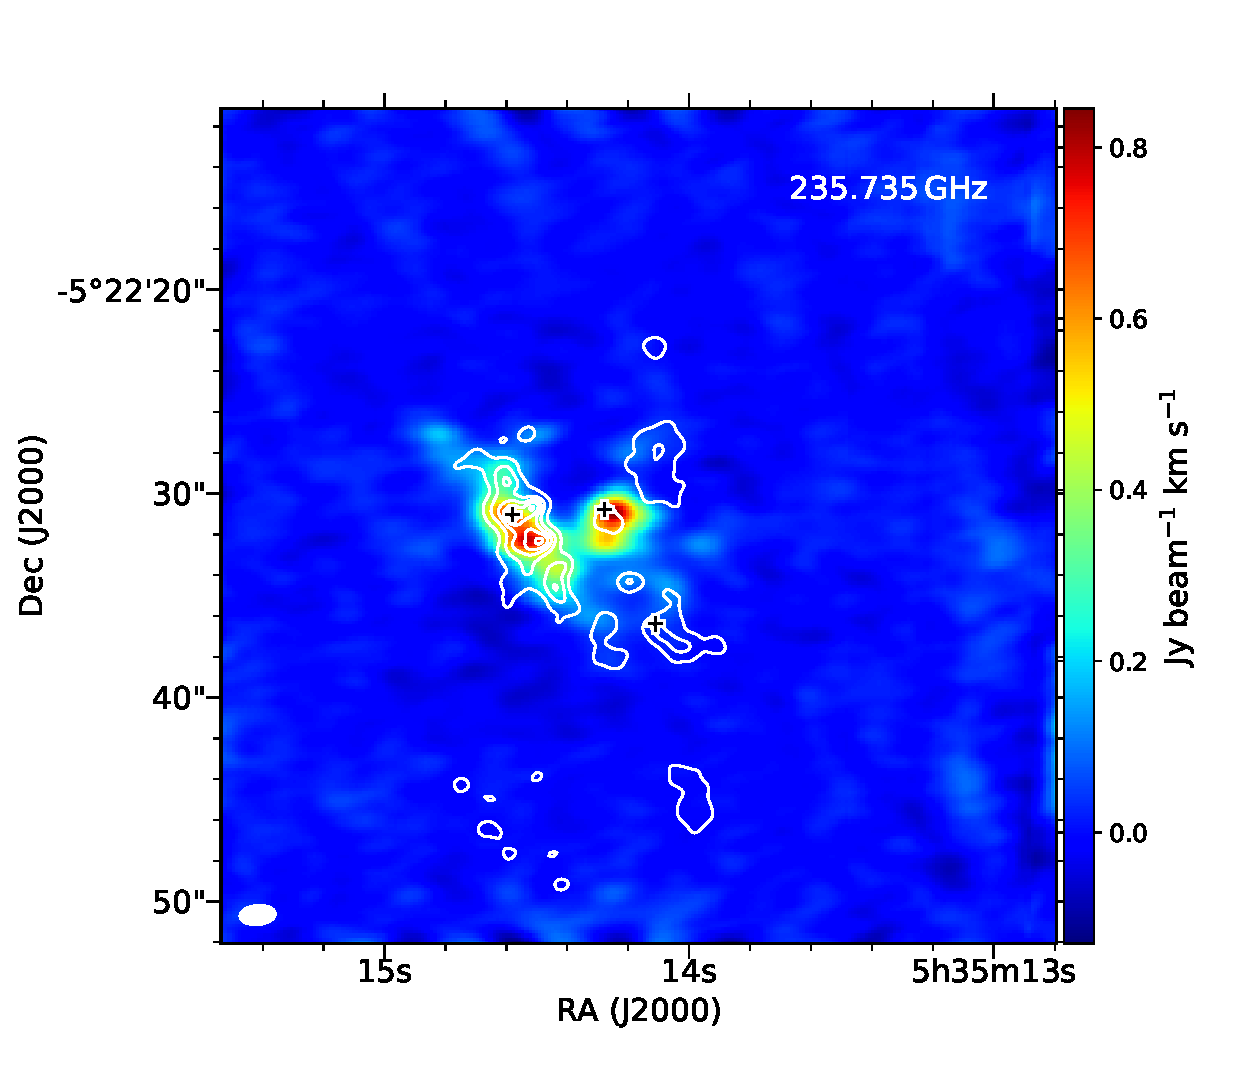
\includegraphics[width=0.98\textwidth]{OrionKL/mom0/235.735mom0_3-7.eps}
%\\(e) 左の図の説明
\end{center}
\end{minipage}
\begin{minipage}{0.48\textwidth}
\begin{center}
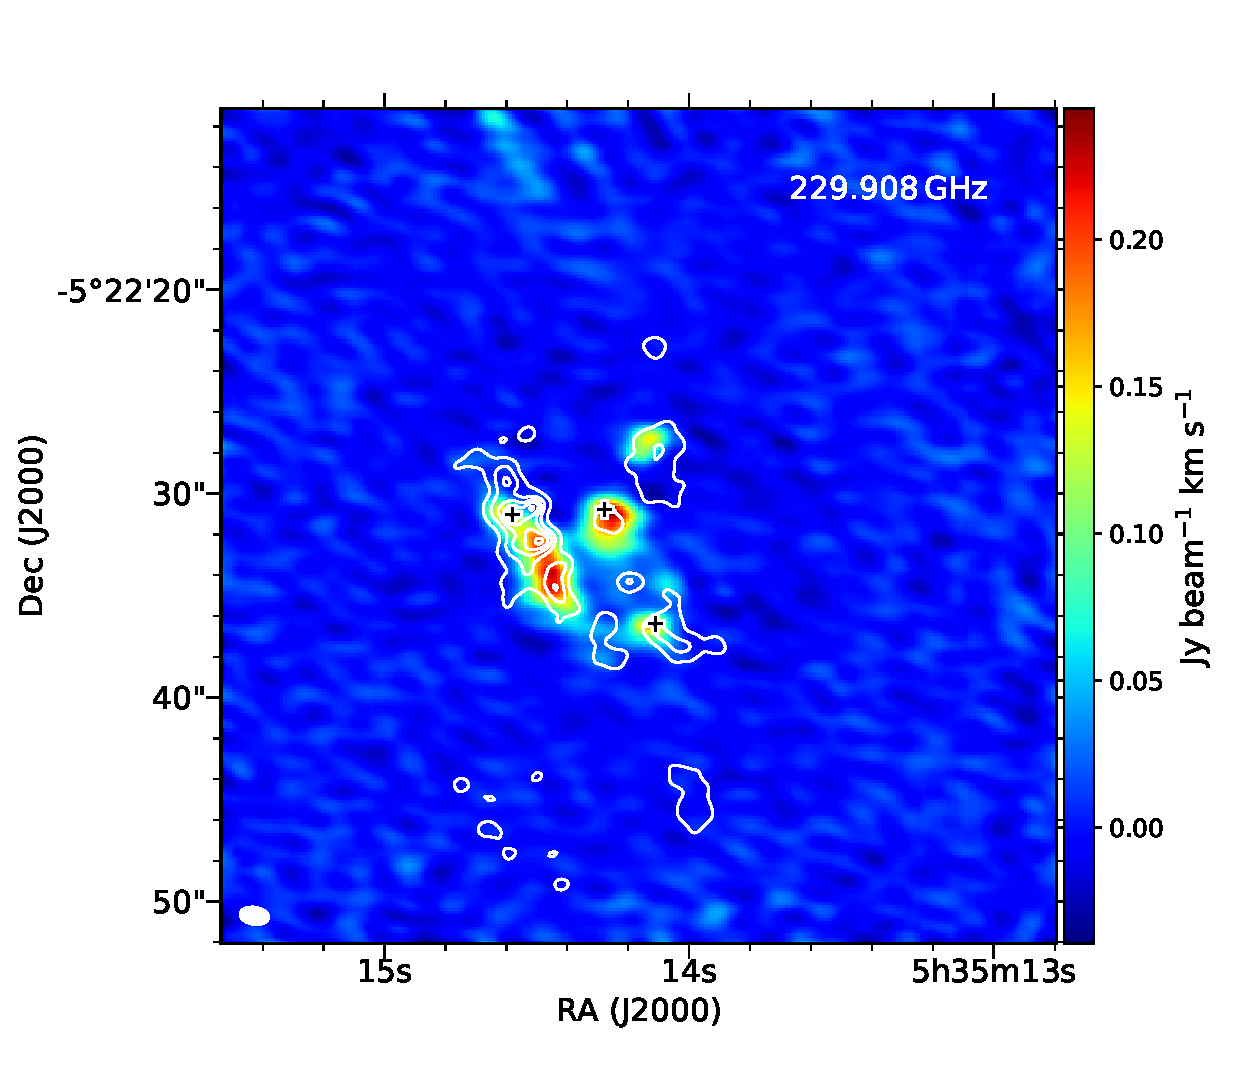
\includegraphics[width=0.98\textwidth]{OrionKL/mom0/229.908mom0_3-7.eps}
%\\(f) 右の図の説明
\end{center}
\end{minipage}
\end{center}
\end{minipage}
%%%% ここまで一組

\begin{minipage}{0.98\textwidth} 
\begin{center}
\begin{minipage}{0.48\textwidth}
\begin{center}
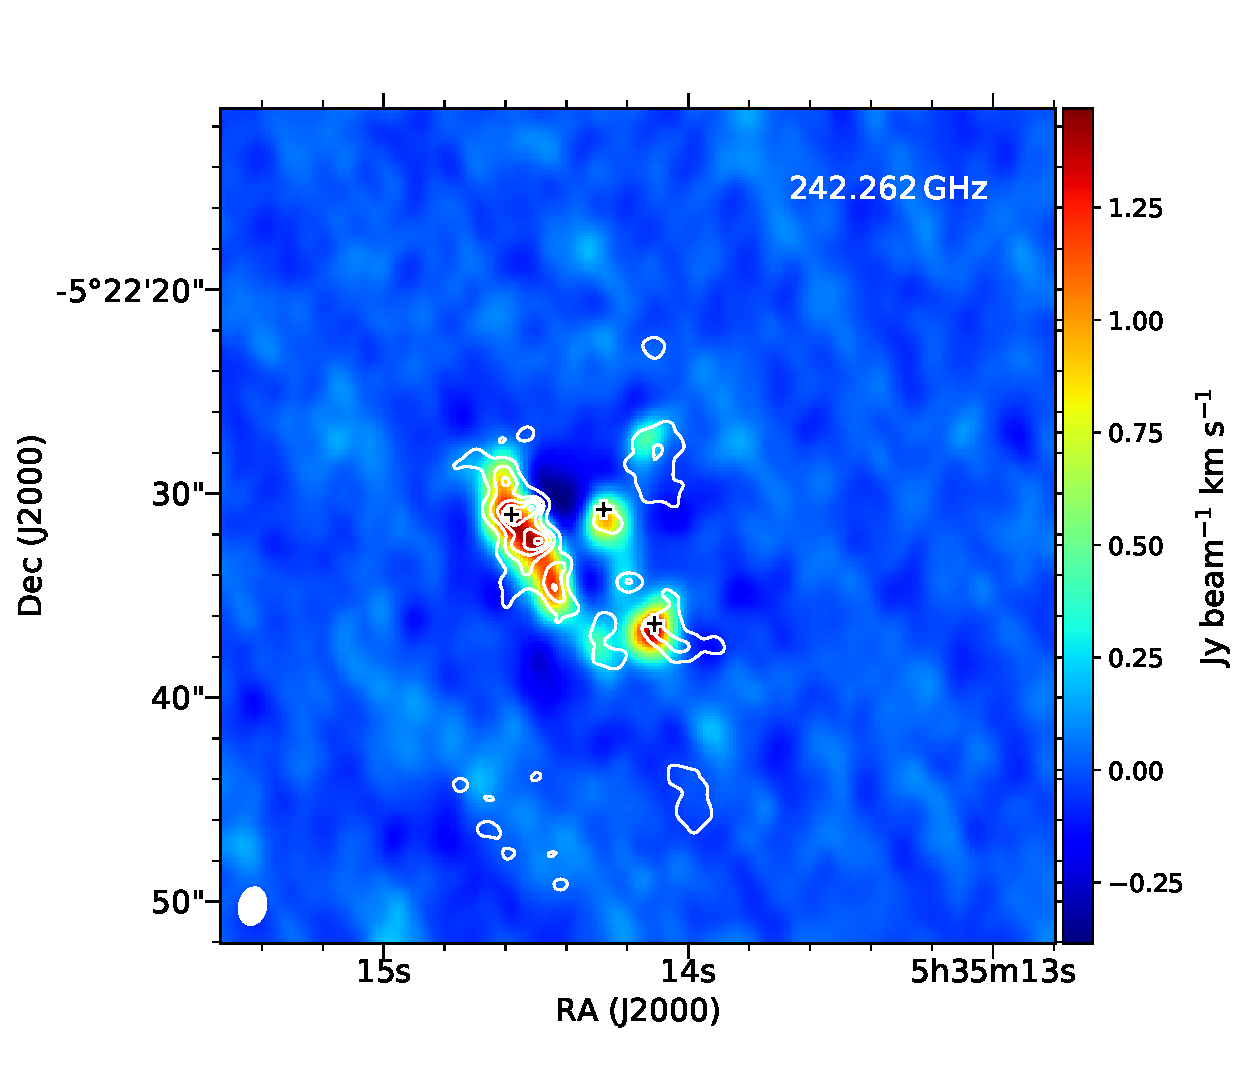
\includegraphics[width=0.98\textwidth]{OrionKL/mom0/242.262SV_mom0_3-7.eps}
%\\(g) 左の図の説明
\end{center}
\end{minipage}
\begin{minipage}{0.48\textwidth}
\begin{center}
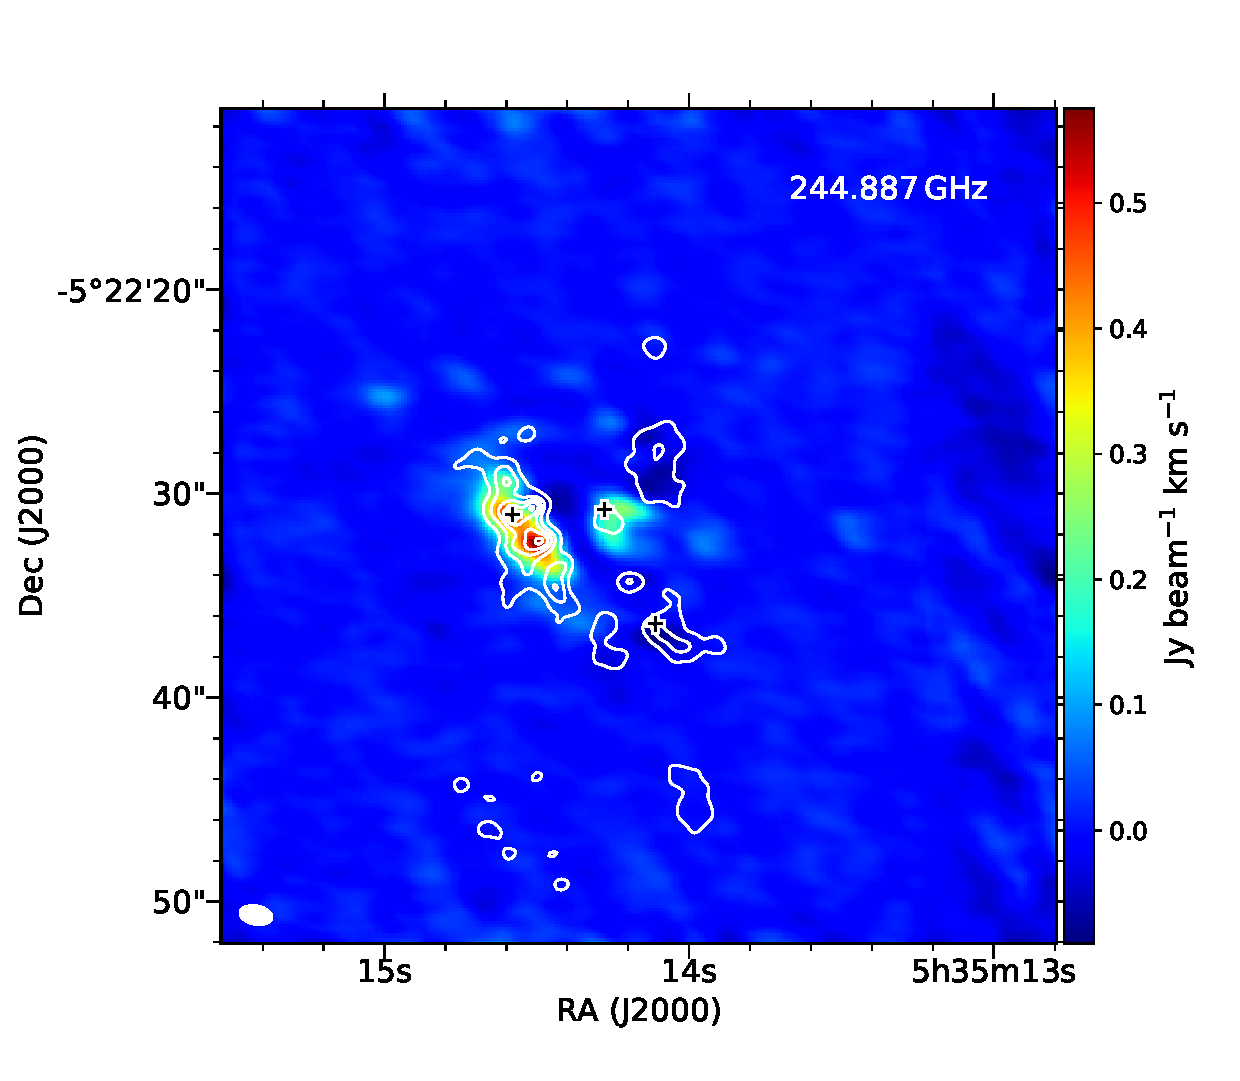
\includegraphics[width=0.98\textwidth]{OrionKL/mom0/244.887mom0_3-7.eps}
%\\(h) 右の図の説明
\end{center}
\end{minipage}
\end{center}
\end{minipage}

\label{fig:mom0s}
\caption{Integrated intensity maps of unblended CH$_{3}$NH$_{2}$ lines. 
The white contours show the 1.3 mm continuum map from \citet{Hirota+2015},
where the contour levels are 10 \%, 30 \%, 50 \%, 70 \%, 90 \% of the peak intensity.
Black crosses denote Hot core, IRc7, and Compact ridge. 
The rest frequency of each transition shows in the upper right part of each panel.}
%\caption{(Continued)}
\end{center}
\end{figure}
%%%%% 積分強度図ここまで %%%%%

%%%%%% チャネルマップここから
\begin{figure}[H]
  \centering
  \includegraphics[width=0.98\textwidth]{OrionKL/chmap/217.758.eps}
  \caption{
  Channel map of expected unblended 217.758 GHz line show multiple velocity-dependent 
  emission peaks: 4-6 km s$^{-1}$ towards Hot core, 7-9km s$^{-1}$ towards IRc7. 
  Magenta crosses denote Hot core, IRc7, and Compact ridge. Same as Figure \ref{fig:mom0s} but for white contours.}
  \label{ch_0}
\end{figure}

\begin{figure}[H]
  \centering
  \includegraphics[width=0.98\textwidth]{OrionKL/chmap/245.202.eps}
  \caption{Channel map of expected unblended 245.202 GHz line.}
  \label{ch_1}
\end{figure}

\begin{figure}[H]
  \centering
  \includegraphics[width=0.98\textwidth]{OrionKL/chmap/235.735.eps}
  \caption{Channel map of expected unblended 235.735 GHz line.}
  \label{ch_2}
\end{figure}

\begin{figure}[H]
  \centering
  \includegraphics[width=0.98\textwidth]{OrionKL/chmap/229.908.eps}
  \caption{Channel map of expected unblended 229.908 GHz line.}
  \label{ch_3}
\end{figure}

\begin{figure}[H]
  \centering
  \includegraphics[width=0.98\textwidth]{OrionKL/chmap/242.262.eps}
  \caption{Channel map of expected unblended 242.262 GHz line.}
  \label{ch_4}
\end{figure}

\begin{figure}[H]
  \centering
  \includegraphics[width=0.98\textwidth]{OrionKL/chmap/244.887.eps}
  \caption{Channel map of expected unblended 244.887 GHz line.}
  \label{ch_5}
\end{figure}

\newpage
\section{Spectra}
The spectrum were extracted from the region of $1''.0$ in diameter around 
Hot core (RA$_{J2000}: 05^{\rm{h}}35^{\rm{m}}14^{\rm{s}}.580$, Dec$_{J2000}:-05^{\circ}22'31''.029$), 
and the Gaussian fitting was performed to obtain FWHM line widths and the mean local standard of 
rest velocity $V_{\mathrm{LSR}}$ of the emission lines.
The line measurements toward Hot core are listed in Table \ref{tab:paraOri}.


The average LSR velocity and FWHM line width are estimated to be 4.84~$\pm$~0.22~km~s$^{-1}$ and 
4.16~$\pm$~0.79~km~s$^{-1}$, respectively.
 $V_{\mathrm{LSR}}$ are consistent with those reported by \citet{Feng+2015} 
 for N-bearing COMs observed toward the Hot core
 (e.g, 4.9~km~s$^{-1}$ for CH$_2$CHCN, 5.1~km~s$^{-1}$ for CH$_3$CH$_2$CN).
On the other hand, $\Delta V_{1/2}$ of CH$_3$NH$_2$ is narrower than those of other molecule in Hot core
\citep[typically 5--15~km~s$^{-1}$,][]{Pagani+2017}.

\renewcommand{\arraystretch}{1.5}
\begin{table}[htb]
\begin{center}

  \caption{CH$_3$NH$_2$ line parameters toward Hot core}
  \label{tab:paraOri}
{\scriptsize
  \begin{tabular}{ccccccl} \hline
   Fequency [GHz]& E$_{\rm{u}}$ [K] &  peak $T_{\mathrm{B}}$\footnotemark[1] [K] & $V_{\mathrm{LSR}}$\footnotemark[1] [km s$^{-1}$] & $\Delta V_{1/2}$\footnotemark[1] [km s$^{-1}$] & Noise [K]  & Note \\ \hline 
    217.758  & 182.05 &  0.86(0.03) & 4.73(0.08) & 3.99(0.24) & 0.034 & \\
    245.202 & 168.31 & 0.37(0.01) & 4.51(0.08) & 3.86(0.33) & 0.037 & \\
    229.908  & 92.71 &  0.65(0.01) & 4.91(0.03) & 3.19(0.06)& 0.064&\\ 
    235.735  & 92.76 & 1.70(0.02) & 4.86(0.03) & 5.60(0.10)& 0.081 & \\
    242.262  & 60.86 &  2.03(0.03) & 4.80(0.09) & 8.04(0.23) & 0.166 & Partially blended \\
    244.887  & 48.09 & 1.29(0.57)& 5.23(0.90) & 4.16(2.12) & 0.043 & \\ \hline
  \end{tabular}
  }
\end{center}
\end{table}
\footnotetext[1]{Numbers in parenthesis represent standard deviation in the unit of the last significant digits.}

Please note that the spectrum in Figure \ref{fig:spec} is superimposed with the result of the Gaussian fitting 
assuming the average $\Delta V_{1/2} = 4.2\, \mathrm{km\,s^{-1}}$.

%%%%% スペクトル挿入 %%%%%
\begin{figure}[H] 
\begin{center}
\begin{minipage}{0.98\textwidth} 
\begin{center}
%%%% ここから
\begin{minipage}{0.48\textwidth}
\begin{center}
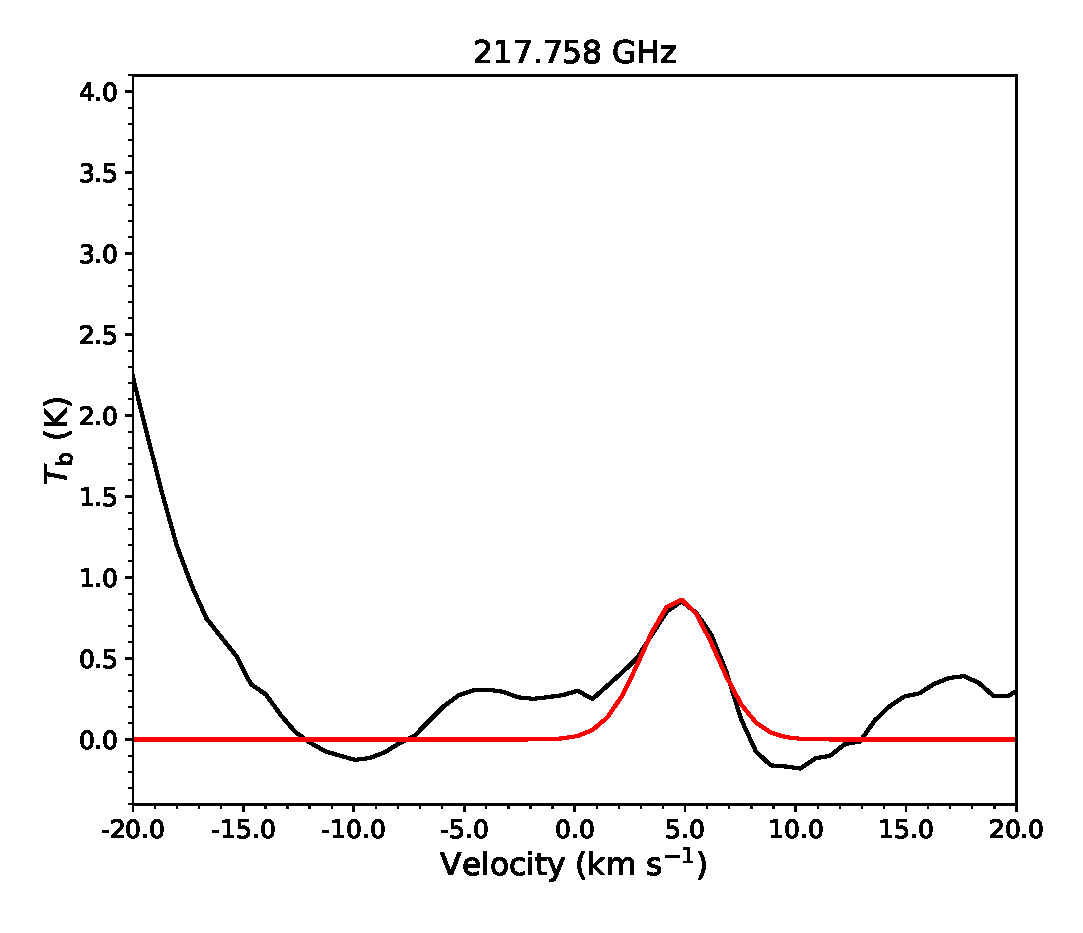
\includegraphics[width=0.98\textwidth]{OrionKL/spectrum/HC/217.758328w_fit.eps}
%\\(a) 左の図の説明
\end{center}
\end{minipage}
\begin{minipage}{0.48\textwidth}
\begin{center}
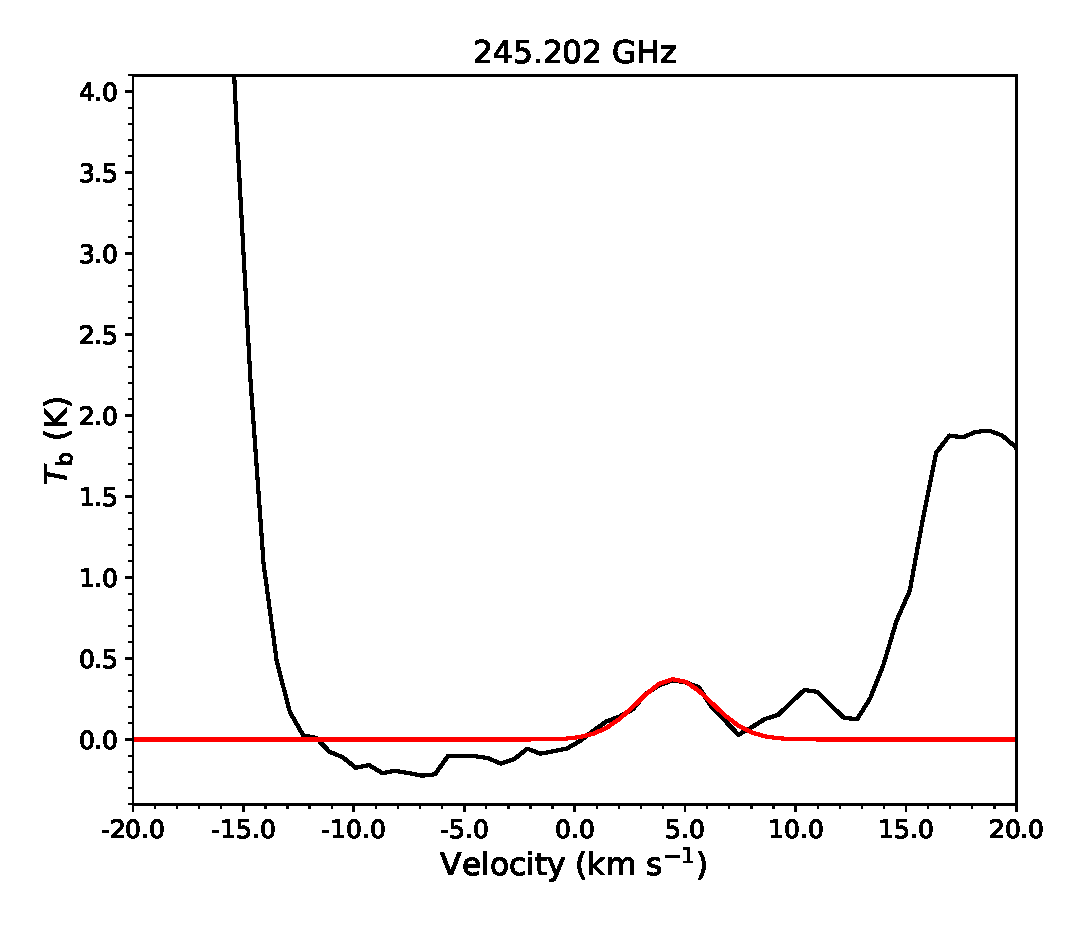
\includegraphics[width=0.98\textwidth]{OrionKL/spectrum/HC/245.2021362w_fit.eps}
%\\(b) 
\end{center}
\end{minipage}
\end{center}
\end{minipage}
%%%% ここまで一組

%\begin{minipage}{0.98\textwidth} 
%\begin{center}
%\begin{minipage}{0.48\textwidth}
%\begin{center}
%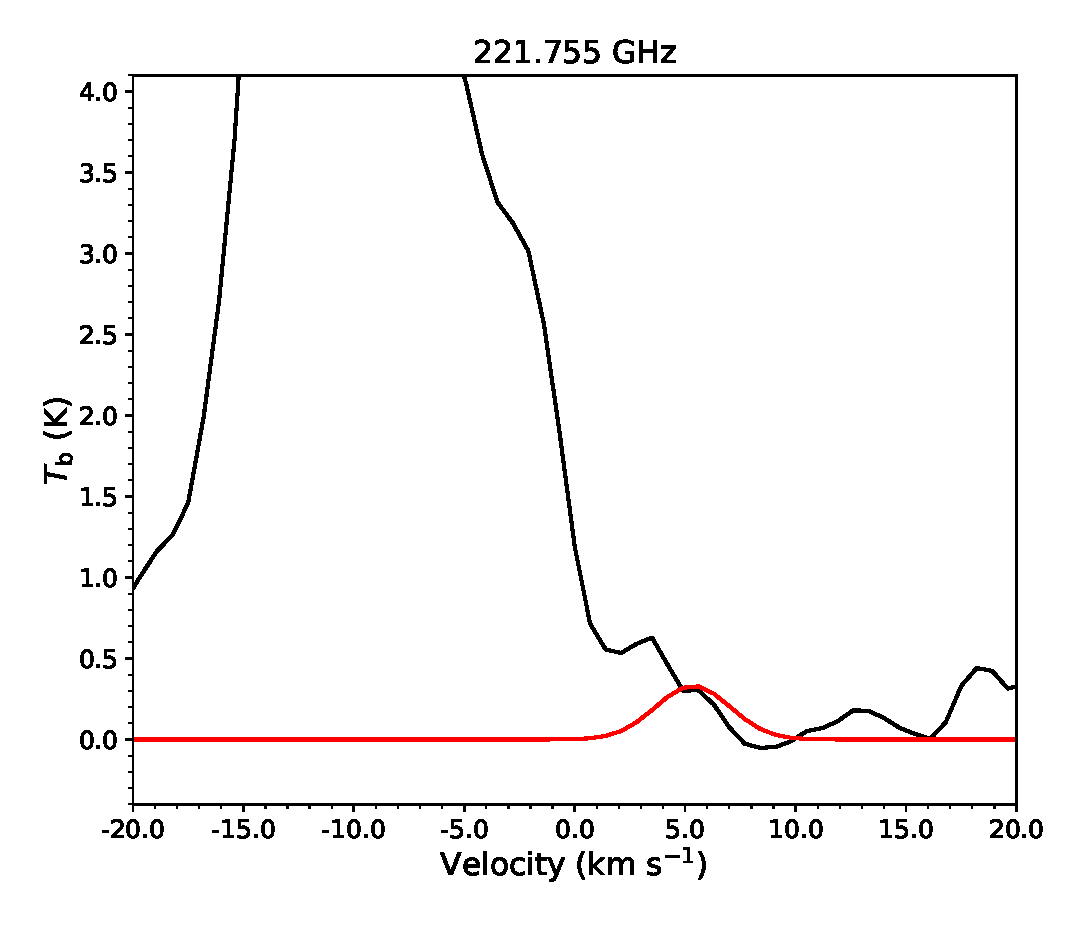
\includegraphics[width=0.98\textwidth]{OrionKL/spectrum/HC/221.755055w_fit.eps}
%\\(c) 左の図の説明
%\end{center}
%\end{minipage}
%\begin{minipage}{0.48\textwidth}
%\begin{center}
%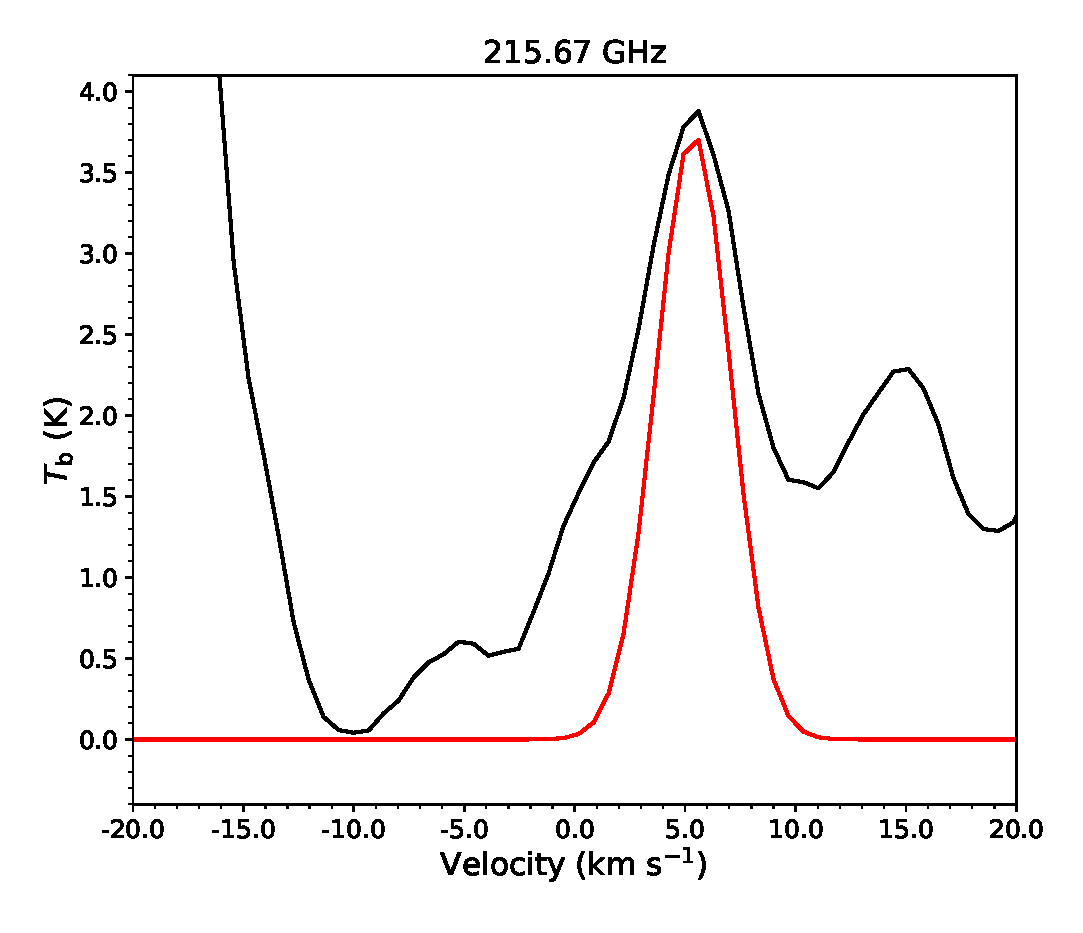
\includegraphics[width=0.98\textwidth]{OrionKL/spectrum/HC/215.6696452w_fit.eps}
%\\(d) 右の図の説明
%\end{center}
%\end{minipage}
%\end{center}
%\end{minipage}
\begin{minipage}{0.98\textwidth} 
\begin{center}
%%%% ここから
\begin{minipage}{0.48\textwidth}
\begin{center}
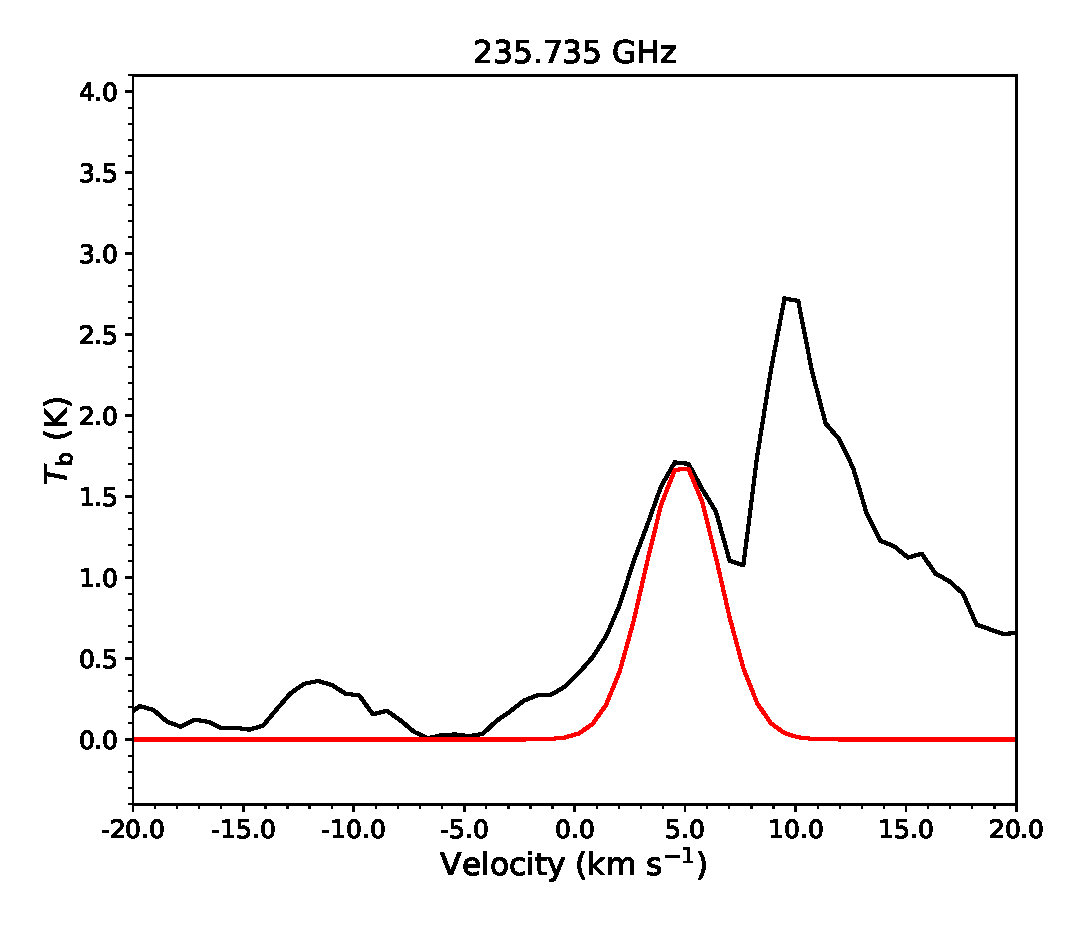
\includegraphics[width=0.98\textwidth]{OrionKL/spectrum/HC/235.735037w_fit.eps}
%\\(e) 左の図の説明
\end{center}
\end{minipage}
\begin{minipage}{0.48\textwidth}
\begin{center}
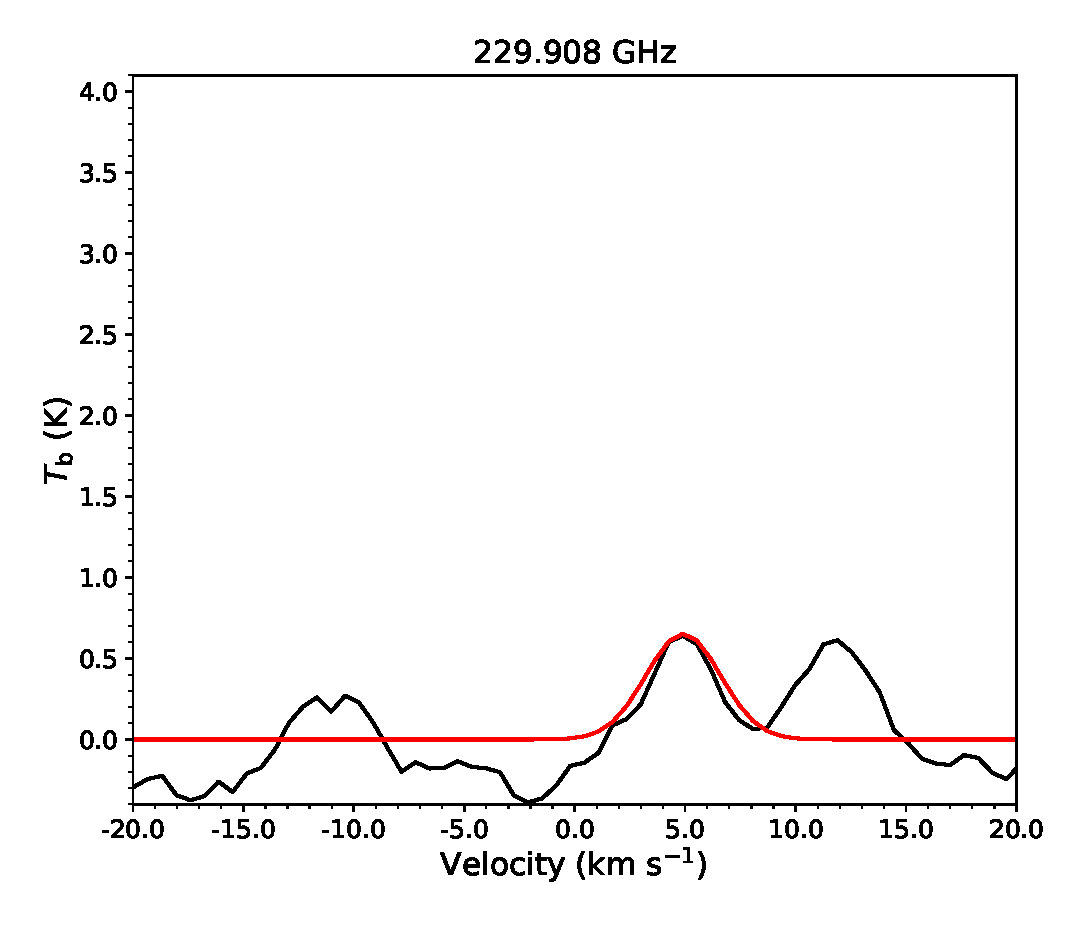
\includegraphics[width=0.98\textwidth]{OrionKL/spectrum/HC/229.908118w_fit.eps}
%\\(f) 右の図の説明
\end{center}
\end{minipage}
\end{center}
\end{minipage}
%%%% ここまで一組

\begin{minipage}{0.98\textwidth} 
\begin{center}
\begin{minipage}{0.48\textwidth}
\begin{center}
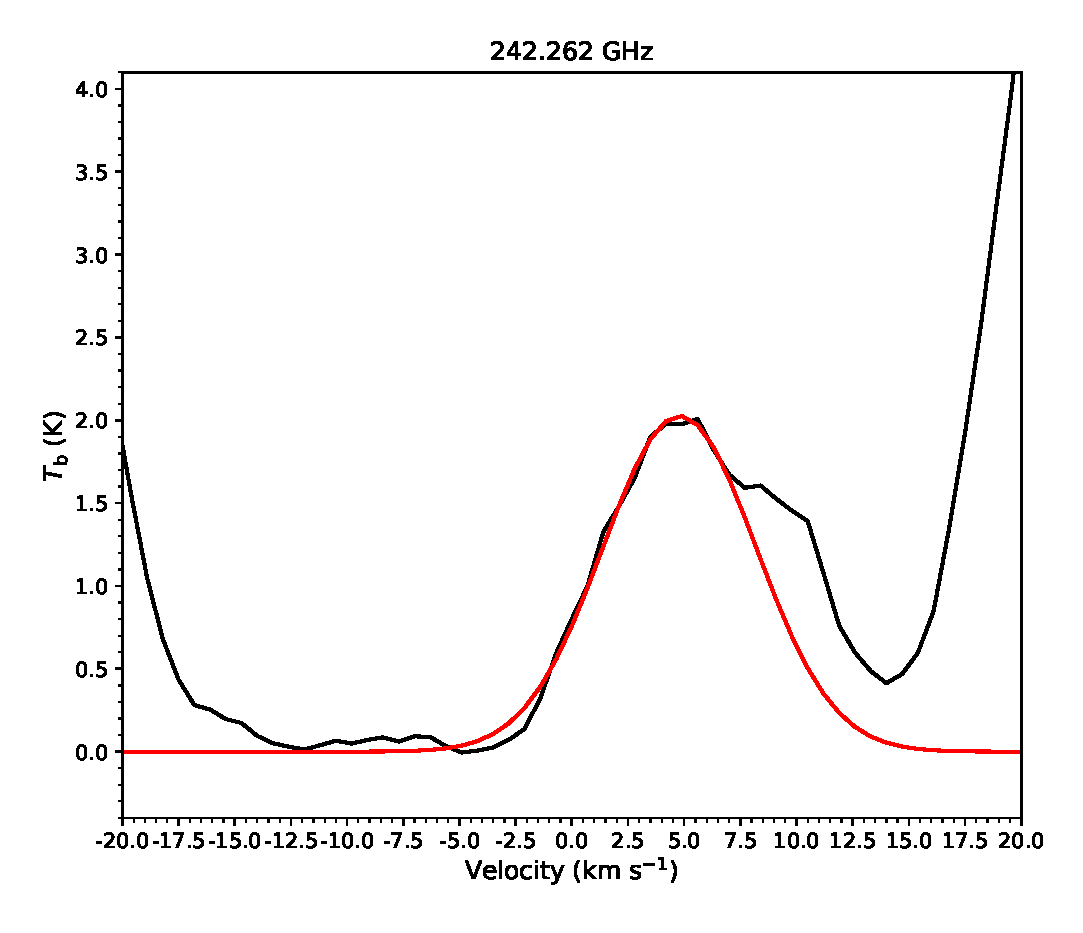
\includegraphics[width=0.98\textwidth]{OrionKL/spectrum/HC/242.2620195w_fit.eps}
%\\(g) 左の図の説明
\end{center}
\end{minipage}
\begin{minipage}{0.48\textwidth}
\begin{center}
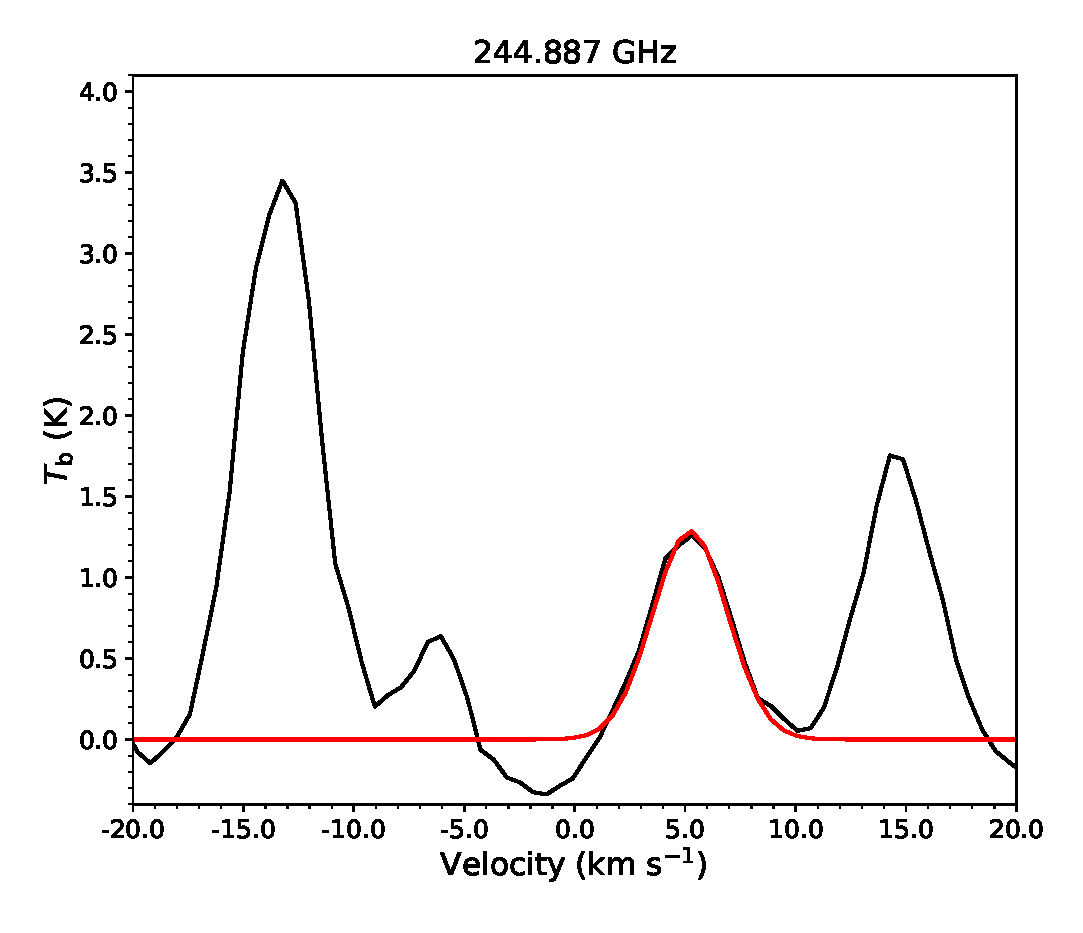
\includegraphics[width=0.98\textwidth]{OrionKL/spectrum/HC/244.8869007w_fit.eps}
%\\(h) 右の図の説明
\end{center}
\end{minipage}
\end{center}
\end{minipage}

\label{fig:spec}
\caption{Spectrum of the CH$_3$NH$_2$ lines at each frequency observed in Hot core center (black) 
 and the result of the Gaussian fitting assuming the average $\Delta V_{1/2} = 4.2\, \mathrm{km\,s^{-1}}$ (red).}
\end{center}
\end{figure}
